% Options for packages loaded elsewhere
\PassOptionsToPackage{unicode}{hyperref}
\PassOptionsToPackage{hyphens}{url}
%
\documentclass[
]{book}
\usepackage{amsmath,amssymb}
\usepackage{iftex}
\ifPDFTeX
  \usepackage[T1]{fontenc}
  \usepackage[utf8]{inputenc}
  \usepackage{textcomp} % provide euro and other symbols
\else % if luatex or xetex
  \usepackage{unicode-math} % this also loads fontspec
  \defaultfontfeatures{Scale=MatchLowercase}
  \defaultfontfeatures[\rmfamily]{Ligatures=TeX,Scale=1}
\fi
\usepackage{lmodern}
\ifPDFTeX\else
  % xetex/luatex font selection
\fi
% Use upquote if available, for straight quotes in verbatim environments
\IfFileExists{upquote.sty}{\usepackage{upquote}}{}
\IfFileExists{microtype.sty}{% use microtype if available
  \usepackage[]{microtype}
  \UseMicrotypeSet[protrusion]{basicmath} % disable protrusion for tt fonts
}{}
\makeatletter
\@ifundefined{KOMAClassName}{% if non-KOMA class
  \IfFileExists{parskip.sty}{%
    \usepackage{parskip}
  }{% else
    \setlength{\parindent}{0pt}
    \setlength{\parskip}{6pt plus 2pt minus 1pt}}
}{% if KOMA class
  \KOMAoptions{parskip=half}}
\makeatother
\usepackage{xcolor}
\usepackage{longtable,booktabs,array}
\usepackage{calc} % for calculating minipage widths
% Correct order of tables after \paragraph or \subparagraph
\usepackage{etoolbox}
\makeatletter
\patchcmd\longtable{\par}{\if@noskipsec\mbox{}\fi\par}{}{}
\makeatother
% Allow footnotes in longtable head/foot
\IfFileExists{footnotehyper.sty}{\usepackage{footnotehyper}}{\usepackage{footnote}}
\makesavenoteenv{longtable}
\usepackage{graphicx}
\makeatletter
\newsavebox\pandoc@box
\newcommand*\pandocbounded[1]{% scales image to fit in text height/width
  \sbox\pandoc@box{#1}%
  \Gscale@div\@tempa{\textheight}{\dimexpr\ht\pandoc@box+\dp\pandoc@box\relax}%
  \Gscale@div\@tempb{\linewidth}{\wd\pandoc@box}%
  \ifdim\@tempb\p@<\@tempa\p@\let\@tempa\@tempb\fi% select the smaller of both
  \ifdim\@tempa\p@<\p@\scalebox{\@tempa}{\usebox\pandoc@box}%
  \else\usebox{\pandoc@box}%
  \fi%
}
% Set default figure placement to htbp
\def\fps@figure{htbp}
\makeatother
\setlength{\emergencystretch}{3em} % prevent overfull lines
\providecommand{\tightlist}{%
  \setlength{\itemsep}{0pt}\setlength{\parskip}{0pt}}
\setcounter{secnumdepth}{5}
\usepackage{booktabs}
\usepackage[]{natbib}
\bibliographystyle{plainnat}
\usepackage{bookmark}
\IfFileExists{xurl.sty}{\usepackage{xurl}}{} % add URL line breaks if available
\urlstyle{same}
\hypersetup{
  pdftitle={Análisis Series de Tiempo: Precio del Oro},
  pdfauthor={Nicolás Méndez Gutiérrez - Christian Martinez},
  hidelinks,
  pdfcreator={LaTeX via pandoc}}

\title{Análisis Series de Tiempo: Precio del Oro}
\author{Nicolás Méndez Gutiérrez - Christian Martinez}
\date{2025-04-28}

\begin{document}
\maketitle

{
\setcounter{tocdepth}{1}
\tableofcontents
}
\chapter{Descripción del dataset}\label{descripciuxf3n-del-dataset}

Este conjunto de datos contiene registros históricos del precio del oro desde el 31 de diciembre de 2013 hasta el 5 de noviembre de 2024, extraídos del mercado MCX. Se trata de un dataset útil para el análisis de series temporales y la predicción de tendencias del precio del oro.

\section{Estructura de los datos}\label{estructura-de-los-datos}

El dataset incluye 2806 entradas y múltiples columnas con información clave:

\begin{itemize}
\tightlist
\item
  Date: Fecha de transacción.
\item
  Open: Precio de apertura del mercado
\item
  High: Precio más alto alcanzado en el día
\item
  Low: Precio más bajo alcanzado en el día
\item
  Price: Precio de cierre del día
\item
  Volume: Cantidad de transacciones realizadas
\item
  Chg\%: Variación porcentual del precio respecto al día anterior.
\end{itemize}

\chapter{Objetivo}\label{objetivo}

Con este dataset se busca analizar el comportamiento histórico de los precios del oro con el objetivo de identificar tendencias significativas a lo largo del tiempo. Además, permite aplicar modelos estadísticos y de aprendizaje automático para predecir movimientos futuros del mercado, proporcionando herramientas útiles para comprender las dinámicas de este activo financiero y apoyar la toma de decisiones en contextos económicos y de inversión.

\chapter{Justificación}\label{justificaciuxf3n}

El dataset de precios diarios del oro es altamente adecuado para la aplicación de técnicas de análisis de series de tiempo debido a las siguientes características:

\begin{enumerate}
\def\labelenumi{\arabic{enumi}.}
\tightlist
\item
  Datos de tiempo ordenados
\end{enumerate}

\begin{itemize}
\tightlist
\item
  La variable Date proporciona una secuencia cronológica continua sin valores faltantes, lo que facilita la modelación de tendencias y patrones temporales.
\item
  La periodicidad diaria permite estudiar el comportamiento del mercado con alta resolución temporal.
\end{itemize}

\begin{enumerate}
\def\labelenumi{\arabic{enumi}.}
\setcounter{enumi}{1}
\tightlist
\item
  Evolución de variable dependiente
\end{enumerate}

\begin{itemize}
\tightlist
\item
  La columna Price representa el precio de cierre, una métrica clave para analizar la evolución del valor del oro a lo largo del tiempo.
\item
  Al ser una serie numérica con cambios graduales y picos específicos, es ideal para aplicar modelos predictivos como ARIMA, modelos de suavizamiento exponencial y redes neuronales recurrentes.
\end{itemize}

\begin{enumerate}
\def\labelenumi{\arabic{enumi}.}
\setcounter{enumi}{2}
\tightlist
\item
  Factores Exógenos y Multivariabilidad
\end{enumerate}

\begin{itemize}
\tightlist
\item
  Las variables Open, High, Low y Volume permiten estudiar la influencia de distintos factores sobre la variación del precio, enriqueciendo el análisis.
\item
  La columna Chg\% proporciona información sobre volatilidad y puede usarse para identificar momentos de alta inestabilidad en el mercado.
\end{itemize}

\begin{enumerate}
\def\labelenumi{\arabic{enumi}.}
\setcounter{enumi}{3}
\tightlist
\item
  Aplicabilidad Real y Relevancia Económica
\end{enumerate}

\begin{itemize}
\tightlist
\item
  El oro es un activo financiero de gran importancia en la economía global, por lo que analizar sus precios a lo largo del tiempo tiene aplicaciones prácticas en predicción de tendencias, evaluación de riesgos y toma de decisiones de inversión.
\item
  Permite la identificación de patrones estacionales, ciclos de mercado y efectos de eventos económicos en la fluctuación del precio.
\end{itemize}

\begin{enumerate}
\def\labelenumi{\arabic{enumi}.}
\setcounter{enumi}{4}
\tightlist
\item
  Calidad de los datos
\end{enumerate}

\begin{itemize}
\tightlist
\item
  Con 2806 registros sin valores faltantes, el dataset proporciona información confiable para entrenar modelos sin la necesidad de una limpieza exhaustiva.
\item
  La estabilidad en la estructura del dataset facilita la aplicación de metodologías estadísticas y de machine learning.
\end{itemize}

En conclusión este dataset es ideal para estudios de series de tiempo, ya que permite aplicar modelos predictivos, evaluar la influencia de factores exógenos y analizar tendencias económicas con datos sólidos y completos.

\chapter{Análisis Exploratorio de Datos}\label{anuxe1lisis-exploratorio-de-datos}

Se importa el dataset cuyos primeros registros se muestran a continuación.

\begin{verbatim}
# A tibble: 6 x 7
  Date       Price  Open  High   Low Volume `Chg%`
  <date>     <dbl> <dbl> <dbl> <dbl>  <dbl>  <dbl>
1 2024-11-06 77030 78300 78570 77030      0  -1.86
2 2024-11-05 78490 78224 78670 78160      0   0.11
3 2024-11-04 78401 78498 78642 78237      0  -0.54
4 2024-11-01 78829 78650 78887 78550      0   0.64
5 2024-10-31 78326 79264 79999 77803     90  -1.17
6 2024-10-30 79257 79119 79375 78888    130   0.5 
\end{verbatim}

A continuación se presenta un resumen de medidas descriptivas.

\begin{table}

\caption{\label{tab:2}Data summary}
\centering
\begin{tabular}[t]{l|l}
\hline
Name & datos\\
\hline
Number of rows & 2806\\
\hline
Number of columns & 7\\
\hline
\_\_\_\_\_\_\_\_\_\_\_\_\_\_\_\_\_\_\_\_\_\_\_ & \\
\hline
Column type frequency: & \\
\hline
Date & 1\\
\hline
numeric & 6\\
\hline
\_\_\_\_\_\_\_\_\_\_\_\_\_\_\_\_\_\_\_\_\_\_\_\_ & \\
\hline
Group variables & None\\
\hline
\end{tabular}
\end{table}

\textbf{Variable type: Date}

\begin{tabular}{l|r|r|l|l|l|r}
\hline
skim\_variable & n\_missing & complete\_rate & min & max & median & n\_unique\\
\hline
Date & 0 & 1 & 2014-01-01 & 2024-11-06 & 2019-05-27 & 2806\\
\hline
\end{tabular}

\textbf{Variable type: numeric}

\begin{tabular}{l|r|r|r|r|r|r|r|r|r|l}
\hline
skim\_variable & n\_missing & complete\_rate & mean & sd & p0 & p25 & p50 & p75 & p100 & hist\\
\hline
Price & 0 & 1 & 40699.89 & 13828.62 & 24545.00 & 29128.00 & 32980.00 & 50613.50 & 79257.0 & ▇▂▃▂▁\\
\hline
Open & 0 & 1 & 40700.22 & 13826.94 & 24583.00 & 29103.75 & 33000.00 & 50646.75 & 79264.0 & ▇▂▃▂▁\\
\hline
High & 0 & 1 & 40917.78 & 13900.47 & 24635.00 & 29261.25 & 33220.50 & 50911.25 & 79999.0 & ▇▂▃▂▁\\
\hline
Low & 0 & 1 & 40482.31 & 13756.09 & 24470.00 & 28974.00 & 32890.00 & 50337.50 & 78888.0 & ▇▂▃▂▁\\
\hline
Volume & 0 & 1 & 12529.58 & 10649.99 & 0.00 & 6282.50 & 10770.00 & 16397.50 & 106920.0 & ▇▁▁▁▁\\
\hline
Chg\% & 0 & 1 & 0.04 & 0.83 & -5.98 & -0.38 & 0.04 & 0.45 & 5.3 & ▁▁▇▁▁\\
\hline
\end{tabular}

Se explora la existencia de datos faltantes.

\begin{verbatim}
  Date  Price   Open   High    Low Volume   Chg% 
     0      0      0      0      0      0      0 
\end{verbatim}

Se realizan gráficos para observar tendencias a lo largo del tiempo de:

\begin{itemize}
\item
  El precio
  \pandocbounded{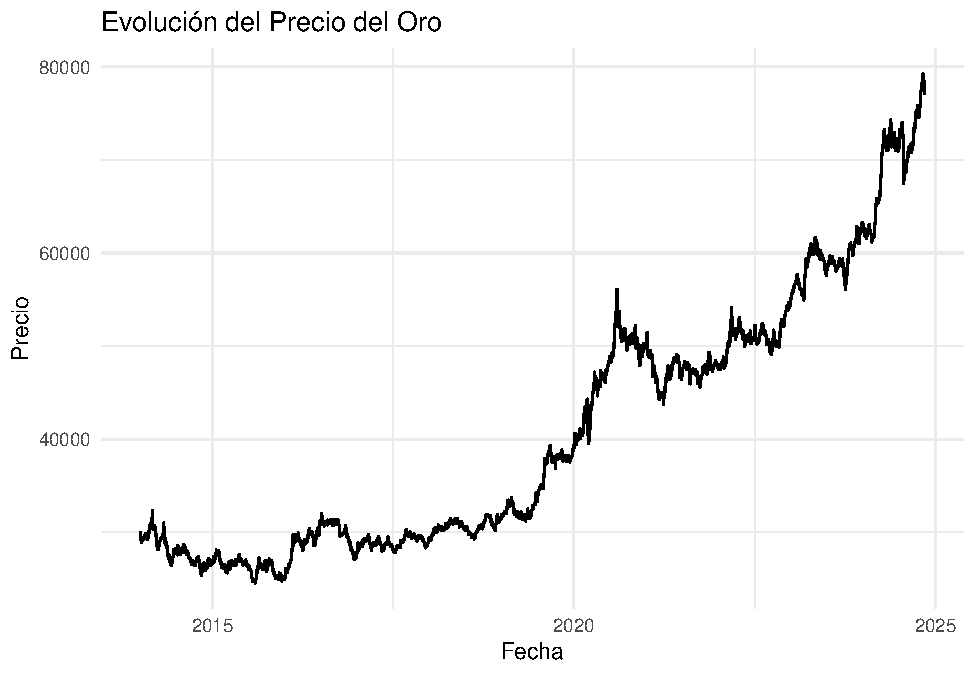
\includegraphics[keepaspectratio]{_main_files/figure-latex/4-1.pdf}}
\item
  Cambios porcentuales
  \pandocbounded{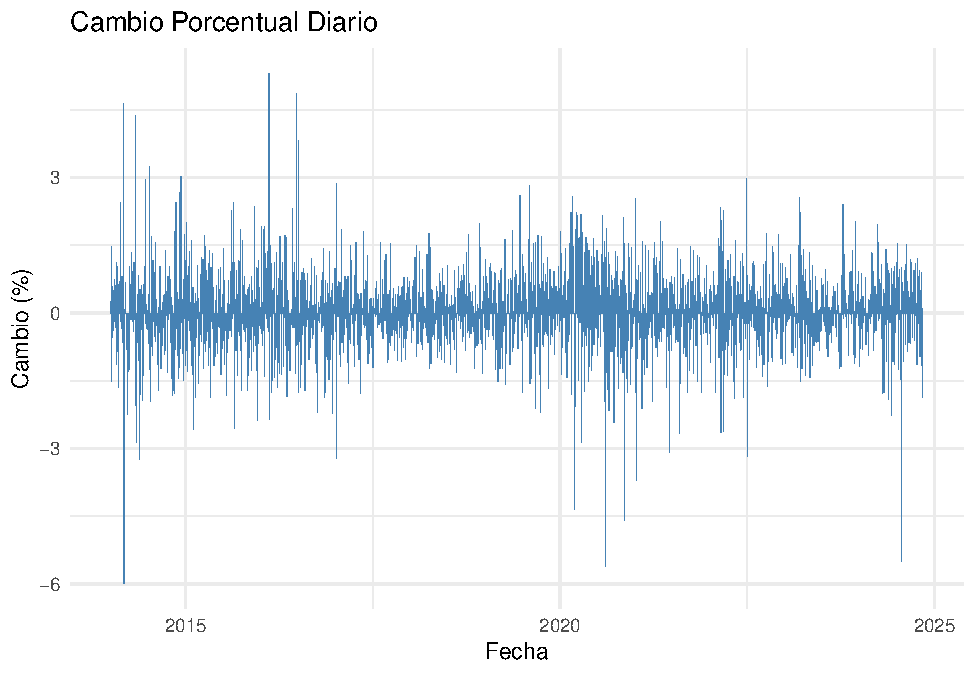
\includegraphics[keepaspectratio]{_main_files/figure-latex/5-1.pdf}}
\item
  Comparación del valor máximo vs mínimos del día
  \pandocbounded{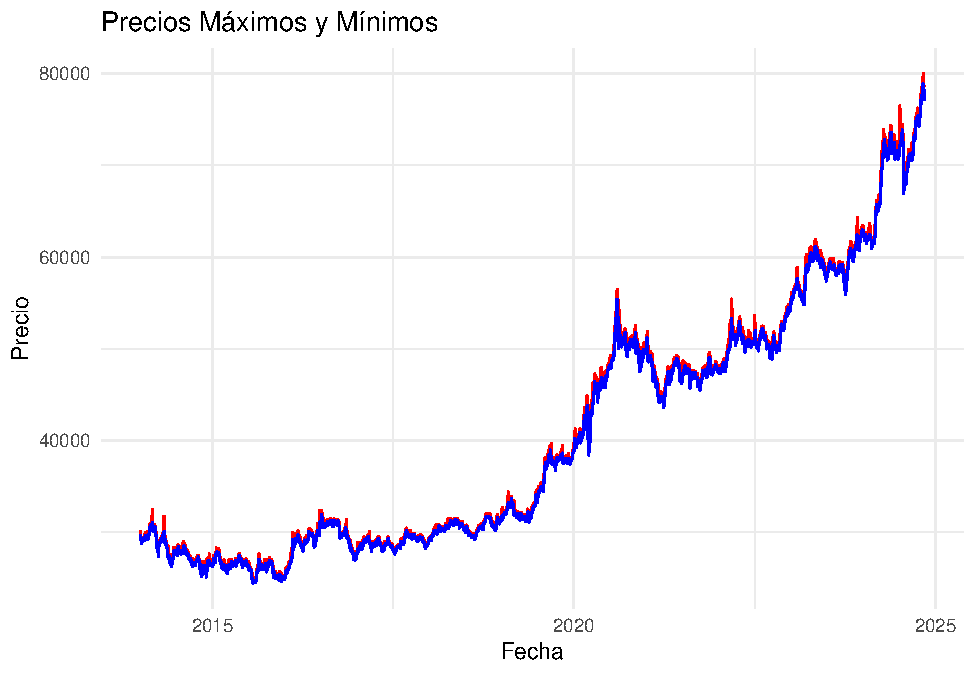
\includegraphics[keepaspectratio]{_main_files/figure-latex/6-1.pdf}}
\end{itemize}

\section{Análisis de promedio movil, rezagos y estacionalidad}\label{anuxe1lisis-de-promedio-movil-rezagos-y-estacionalidad}

\subsection{Promedio móvil}\label{promedio-muxf3vil}

Se agrega un promedio móvil de 7 días, es decir, de manera semanal ya que muchos mercados (como el oro, acciones, productos básicos) tienden a mostrar variaciones semanales
(por factores como fin de semana, cierres de mercado, ciclos de noticias, etc.)

\pandocbounded{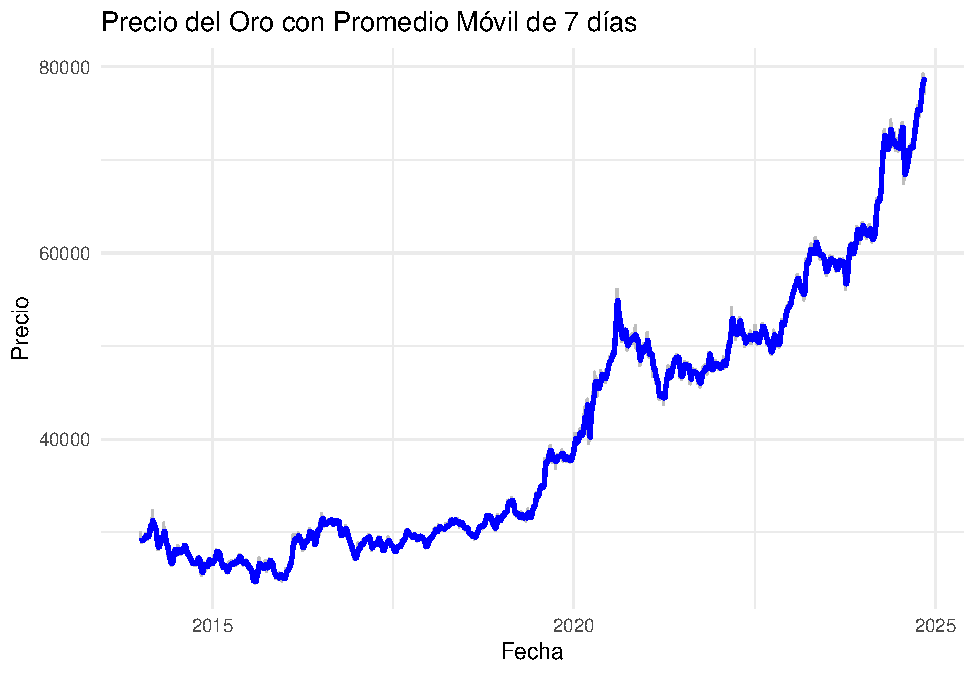
\includegraphics[keepaspectratio]{_main_files/figure-latex/8-1.pdf}}

Se hacen las siguientes observaciones:

\begin{itemize}
\tightlist
\item
  La serie muestra una tendencia creciente de largo plazo, especialmente desde 2019 en adelante.
\item
  2013 - 2018: El precio del oro estuvo relativamente estable o ligeramente a la baja, con pequeñas fluctuaciones.
\item
  2019 - 2020: Se observa un fuerte crecimiento, con un aumento pronunciado en el precio.
\item
  2020 - 2021: Hay una corrección o caída parcial, después de un máximo.
\item
  2021 - 2025: Retoma una tendencia alcista constante con algunos ciclos de subida y bajada.
\item
  Se identifican momentos donde la curva cambia de pendiente (subidas abruptas o correcciones), que pueden estar asociadas a eventos macroeconómicos.
\end{itemize}

\subsection{Rezagos (lags)}\label{rezagos-lags}

\pandocbounded{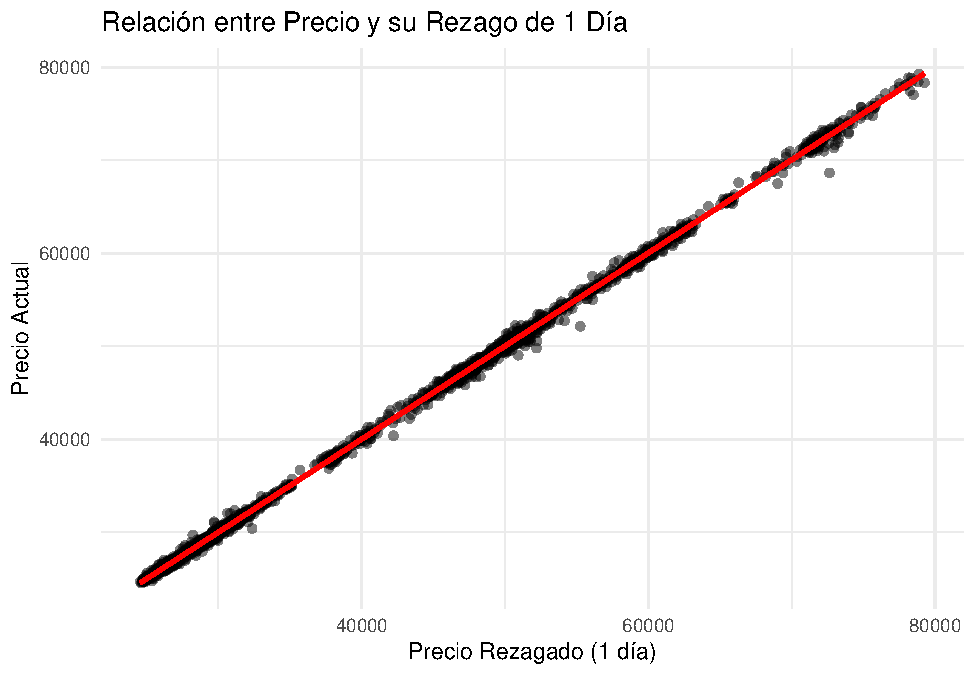
\includegraphics[keepaspectratio]{_main_files/figure-latex/9-1.pdf}}

Se realizan las siguientes observaciones:

\begin{itemize}
\tightlist
\item
  El precio del oro no cambia drásticamente de un día para otro; más bien tiende a seguir la misma trayectoria.
\item
  Hay baja volatilidad diaria relativa (aunque a largo plazo se observaron tendencias importantes).
\end{itemize}

\subsection{Estacionalidad}\label{estacionalidad}

\pandocbounded{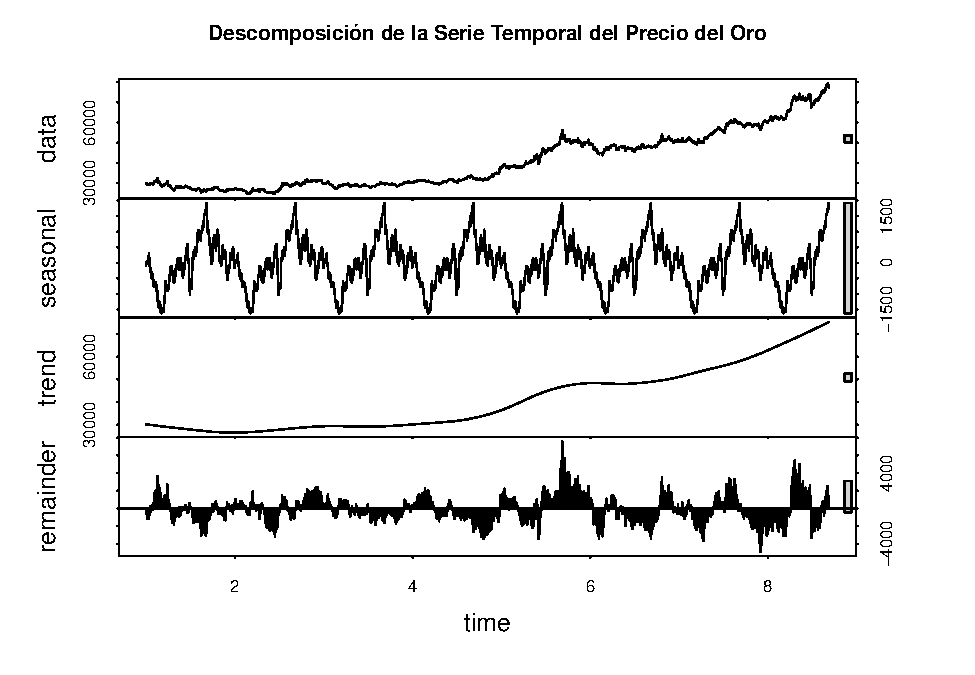
\includegraphics[keepaspectratio]{_main_files/figure-latex/10-1.pdf}}

\begin{itemize}
\tightlist
\item
  En la primera porción de la gráfica, se observa el comportamiento de la variable precio a lo largo del tiempo.
\item
  La segunda porción, Seasonal, muestra cómo varía sistemáticamente a lo largo del año.
\item
  La tercera porción, muestra la Tendencia a largo plazo.
\item
  Finalmente, se observa en la porción de Remainder el ruido no se explicado por la estacionalidad.
\end{itemize}

De la gráfica, se realizan las siguientes observaciones:

\begin{itemize}
\tightlist
\item
  Se aprecia claramente la tendencia creciente fuerte, especialmente desde el año 2020 en adelante.
\item
  El componente estacional muestra ciclos repetitivos con una frecuencia regular de picos y valles aproximadamente cada año. La amplitud del patrón estacional es pequeña en comparación al nivel del precio.
\end{itemize}

\chapter{Fuentes}\label{fuentes}

\begin{itemize}
\tightlist
\item
  Dataset: \url{https://www.kaggle.com/datasets/nisargchodavadiya/daily-gold-price-20152021-time-series}
\end{itemize}

  \bibliography{book.bib}

\end{document}
